\newpage
\chapter{TINJAUAN PUSTAKA} \label{Bab II}

\section{Tinjauan Pustaka} \label{II.Tinjauan}
Sebagai acuan untuk tugas akhir ini, bagian ini akan membahas beberapa penelitian sebelumnya. Penelitian-penelitian yang diulas ini memiliki kaitan dengan masalah dan solusi yang dibahas dalam laporan ini.

\begin{enumerate}[noitemsep]
	\item Penelitian oleh Siddhad et al. (2024) memperkenalkan DrowzEE-G-Mamba, yang merupakan studi \textit{state-of-the-art} (SOTA) terdekat karena menjadi satu-satunya yang menerapkan arsitektur Mamba untuk deteksi kantuk. Penelitian ini menggunakan dataset SEED-VIG dan mencapai akurasi 83,24\%. Metodenya memanfaatkan blok SS-Conv-SSM dan mekanisme 2D selective scan. Model ini dicatat cocok untuk implementasi real-time karena mampu mengurangi false positives dengan tetap mempertahankan akurasi \cite{Siddhad2024}.

	\item Studi oleh Wang et al. (2025) mengusulkan EEGMamba, dasar model EEG pertama yang berbasis Mamba. Model ini menggunakan encoder Mamba \textit{bidirectional} untuk memodelkan dependensi \textit{spatiotemporal}. EEGMamba di \textit{pre-train} menggunakan rekonstruksi \textit{masked} EEG pada korpus data yang sangat besar dari lima dataset dan diberikan enam tugas dengan hilir yang berbeda dijalankan sebagai evaluasi. Keenam tugas tersebut adalah \textit{Emotion Recognition}, \textit{Motor Imagery Classification}, \textit{Sleep Staging}, \textit{Seizure Detection}, \textit{Imagined Speech Classificaiton}, dan \textit{Major Depressive Disorder Diagnosis}. Hasilnya menunjukkan bahwa EEGMamba mencapai kinerja SOTA di semua tugas. Secara khusus, model ini terbukti mengungguli model foundation berbasis Transformer, terutama dalam skenario \textit{low-resource} \cite{Zhou2025}.

	\item Dalam penelitian BiT-MamSleep secara spesifik mengatasi masalah klasifikasi tahap tidur, sebuah tugas yang sangat terkait dengan deteksi kantuk. Penelitian ini mengusulkan arsitektur baru yang menggabungkan Triple-Resolution CNN (TRCNN) untuk ekstraksi fitur multi-skala dengan mekanisme Bidirectional Mamba (BiMamba) untuk memodelkan dependensi temporal jangka panjang. Model ini juga menggunakan Focal Loss dan SMOTE untuk menangani masalah data tidak seimbang. Hasil evaluasi ekstensif pada empat dataset publik menunjukkan bahwa BiT-MamSleep secara signifikan mengungguli metode SOTA sebelumnya \cite{Zhou2024Sleep}.

	\item Penelitian oleh Cao et al. (2025) menjadi benchmark SOTA utama yang secara spesifik menggunakan dataset DROZY. Mereka mengusulkan metode deteksi kantuk multimodal yang mengintegrasikan sinyal fisiologis (EEG, ECG) dan gambar wajah. Model unggulan mereka, "multimodal feature coupled model" menggunakan ResNet18 untuk fitur gambar dan LSTM untuk fitur time-series (EEG/ECG). Keunikan model ini adalah fitur dari modalitas yang berbeda tidak hanya digabungkan, tetapi digunakan sebagai \textit{mutual weights} untuk saling memengaruhi kontribusi akhir. Dengan pendekatan ini, mereka berhasil mencapai akurasi 98,41\% dalam mengklasifikasikan 3 kategori kantuk (Alert, Low Vigilance, Drowsy) pada dataset DROZY \cite{Cao2025Optimized}.

	\item \textit{Review} oleh Li \& Chung (2022)  merangkum lanskap penelitian deteksi kantuk berbasis EEG secara komprehensif. Tinjauan ini mengonfirmasi bahwa sinyal EEG adalah indikator kantuk yang paling andal, mengungguli sinyal fisiologis lainnya. Hasil tinjauan ini menyoroti beberapa tantangan utama yang belum terpecahkan dalam bidang ini. Tantangan terbesar adalah kemampuan generalisasi, karena sinyal EEG sangat bervariasi antar individu, dan penelitian mengenai model yang lintas subjek masih sangat langka. Selain itu, disimpulkan bahwa untuk deteksi dini, model dengan output kontinu seperti regresi lebih baik daripada klasifikasi diskrit \cite{Wang2022}.
\end{enumerate}

Ringkasan penelitian terdahulu dapat dilihat pada Tabel 2.1 berikut.\par
\begin{longtable}{| b{0.05\textwidth}|p{0.2\textwidth}|p{0.2\textwidth}|p{0.15\textwidth}|p{0.25\textwidth}|} % Longtable berguna agar tabel dapat terpotong di halaman baru
	\caption{Literasi Penelitian Terdahulu}
	\label{table:2.literasi}\\
	\hline
	\textbf{No.} & \textbf{Judul} & \textbf{Masalah} & \textbf{Metode} & \textbf{Hasil} \\
	\hline
	\endfirsthead % Header tabel untuk halaman pertama
	\hline
	\textbf{No.} & \textbf{Judul} & \textbf{Masalah} & \textbf{Metode} & \textbf{Hasil} \\
	\hline
	\endhead % Header tabel untuk halaman selanjutnya (repeat header row)
	1. & DrowzEE-G-Mamba: Leveraging EEG and State Space Models for Driver Drowsiness Detection & Deteksi kantuk menggunakan EEG pada dataset SEED-VIG & Arsitektur Mamba (SS-Conv-SSM blocks) & Mencapai akurasi 83,24\%.\\ 
	\hline
	2. & EEGMamba: An EEG foundation model with Mamba & Kebutuhan akan model dasar (foundation model) yang dapat digeneralisasi untuk berbagai tugas EEG (termasuk sleep staging) & Arsitektur Mamba sebagai foundation model yang di-pre-train pada 5 dataset publik & Model Mamba terbukti unggul (SOTA) di berbagai tugas EEG, menunjukkan keefektifannya untuk sinyal sekuensial EEG\\ 
	\hline
	3. & BiT-MamSleep: Bidirectional Temporal Mamba for EEG Sleep Staging & Klasifikasi tahap tidur (sleep staging), sebuah tugas yang sangat mirip dengan deteksi kantuk & Bidirectional Mamba (BiMamba) dikombinasi-kan dengan TRCNN (Triple-Resolution CNN) & Secara signifikan mengungguli SOTA pada 4 dataset tahap tidur publik\\ 
	\hline
	4. & Optimized driver fatigue detection method using multimodal neural networks & Deteksi kantuk multimodal pada dataset DROZY & Multimodal Feature Coupled Model: Menggabung-kan fitur EEG, ECG, dan gambar wajah, mengguna-kan ResNet18 dan LSTM & Mencapai akurasi 98,41\% untuk klasifikasi 3 kategori (\textit{Alert, Low Vigilance, Drowsy}) pada dataset DROZY\\
	\hline
	5. & Electroence-phalogram Based Approaches for Driver Drowsiness Detection and Management A Review & Merangkum berbagai pendekatan dan tantangan dalam deteksi kantuk berbasis EEG & Tinjauan Sistematis (Review) & Mengidentifikasi metode-metode yang ada (seperti CNN, LSTM) dan menyoroti tantangan generalisasi cross-subject\\
	\hline
\end{longtable}

\section{Dasar Teori} \label{II.Teori}
Berikut dipaparkan kerangka teori yang mendasari penelitian ini, khususnya terkait dengan metode klasifikasi kantuk menggunakan sinyal EEG dan EOG. \par

\subsection{Klasifikasi Kantuk} \label{II.Teori1}
Kantuk didefinisikan sebagai keadaan perantara antara terjaga dan tidur yang ditandai dengan penurunan kesadaran progresif serta keinginan kuat untuk tidur \cite{slater2008definition}. Dalam konteks klasifikasi, sangat penting untuk membedakan kantuk dari kelelahan. Karena kelelahan adalah keengganan melanjutkan tugas akibat kerja fisik atau pengalaman berkepanjangan yang membaik dengan istirahat, sedangkan istirahat dan ketidakaktifan justru dapat memperburuk rasa kantuk.

Klasifikasi kantuk bertujuan untuk memetakan kondisi penurunan kewaspadaan ini ke dalam tingkatan yang terukur secara objektif. Dalam studi simulasi berkendara, tingkatan kantuk ini sering dibagi menjadi skala kontinu yang terdiri dari lima kelas deskriptor, yaitu waspada, sedikit mengantuk, cukup mengantuk, sangat mengantuk, hingga ekstrem mengantuk. Validasi klasifikasi ini umumnya didasarkan pada observasi visual terhadap indikator fisik subjek, seperti perubahan nada wajah, pergerakan mata atau penutupan kelopak mata yang lambat, serta perilaku spesifik lainnya \cite{khushaba2011driver}.

\subsection{Sinyal Fisiologis} \label{II.Teori1}
Sinyal fisiologis, yang mencakup pengukuran aktivitas sistem saraf pusat  dan sistem saraf otonom, dianggap sebagai indikator paling akurat untuk klasifikasi kantuk karena mampu mendefinisikan transisi fisiologis antara kondisi terjaga dan tidur secara presisi. Dalam konteks klasifikasi tingkat kantuk ditentukan dengan memantau penyimpangan parameter sinyal dari kondisi waspada, seperti peningkatan daya gelombang otak alpha dan theta pada EEG, penurunan detak jantung yang disertai peningkatan variabilitas detak jantung (HRV) pada ECG, serta peningkatan durasi dan frekuensi kedipan mata pada EOG \cite{8293771}.

\subsubsection{Electroencephalogram (EEG)} \label{II.Teori1.1}
Electroencephalogram (EEG) adalah metode pemantauan neurofisiologis yang merekam dinamika jaringan saraf otak, yang secara alami bersifat non-linear dan non-stasioner. Dalam konteks sistem deteksi kantuk pengemudi, sinyal EEG dianggap sebagai sumber data yang paling menjanjikan dan akurat dibandingkan metode lain seperti pelacakan mata atau perilaku kendaraan, karena kemampuannya untuk mendeteksi transisi keadaan internal otak secara langsung dari sadar menuju tidur. Sinyal ini sangat krusial karena fitur yang diekstraksi dari EEG menunjukkan pola yang konsisten baik untuk kantuk maupun kelelahan, menjadikannya dasar yang andal untuk membangun sistem peringatan dini bagi pengemudi \cite{s21113786}.

Hubungan antara EEG dan klasifikasi tingkat kantuk didasarkan pada perubahan signifikan pola sinyal otak, di mana transisi menuju kelelahan umumnya berkorelasi dengan aktivitas pada pita frekuensi theta dan delta, serta fenomena atenuasi gelombang alpha yang membedakan kondisi terjaga santai dengan permulaan tidur \cite{JIAO2020100}. Selain perubahan pada pita frekuensi, klasifikasi kantuk juga dapat dideteksi melalui perubahan topologi konektivitas fungsional otak yang bergeser dari konfigurasi linear saat waspada menjadi konfigurasi berbentuk bintang saat mengantuk, terutama pada pita alpha dan beta \cite{s21113786}.

\subsubsection{Electrooculogram (EOG)} \label{II.Teori1.1}
Electrooculogram (EOG) adalah sinyal elektrofisiologis yang dihasilkan oleh polarisasi bola mata, yang mencerminkan potensial istirahat antara kornea dan retina. Sinyal ini diukur melalui elektroda yang ditempatkan pada kulit di sekitar mata, di mana magnitudonya bervariasi sesuai dengan perpindahan bola mata dari posisi istirahatnya \cite{malmivuo1995bioelectromagnetism}. Secara teknis, turunan pertama dari sinyal EOG sebanding dengan kecepatan gerakan bola mata, yang memungkinkan analisis dinamika pergerakan mata secara detail. Amplitudo sinyal EOG umumnya berkisar antara 0,4 hingga 10 mV dengan frekuensi bervariasi dari 0,1 hingga 38 Hz, meskipun komponen frekuensi utamanya biasanya berada di bawah 10 Hz, sehingga EOG juga dapat dianggap sebagai bentuk elektromiografi dari otot-otot di sekitar mata \cite{SONG2020101865}.

Dalam konteks klasifikasi tingkat kantuk, EOG digunakan untuk mendeteksi transisi dari kondisi waspada ke mengantuk melalui perubahan pola pergerakan mata dan karakteristik kedipan. Saat seseorang dalam kondisi waspada, sinyal EOG menunjukkan dominasi \textit{Rapid Eye Movements} (REM), sedangkan kondisi kantuk atau permulaan tidur ditandai dengan munculnya \textit{Slow Eye Movements} (SEM) \cite{4977181}. Selain itu, indikator fisiologis yang diekstraksi dari EOG, seperti \textit{Average Blink Time} (ABT) dan \textit{Wavelet Packet Barycenter Frequency} (WPBF), memiliki korelasi signifikan dengan tingkat kelelahan. Studi menunjukkan bahwa seiring meningkatnya kelelahan visual otot (\textit{Muscular Visual Fatigue}), waktu kedipan rata-rata (ABT) akan meningkat secara signifikan sementara frekuensi barycenter (WPBF) akan menurun \cite{SONG2020101865}.

\subsection{Pra-pemrosesan Sinyal} \label{II.Teori1.1}
Pra-pemrosesan sinyal adalah serangkaian langkah awal yang sangat krusial dalam analisis EEG maupun EOG untuk membersihkan data mentah yang seringkali penuh dengan gangguan (\textit{noise}). Proses ini bertujuan memisahkan aktivitas otak yang murni dari artefak yang tidak diinginkan. Sehingga karakteristik sinyal menjadi lebih jelas dan siap diolah. Hal ini mutlak diperlukan karena kualitas penerapan metode pra-pemrosesan akan sangat menentukan akurasi hasil analisis data selanjutnya. Jika sinyal masih kotor, kesimpulan yang diambil dari penelitian bisa menjadi tidak valid \cite{Kim2018}. 

\subsubsection{Segmentasi Sinyal}
Segmentasi sinyal adalah proses mempartisi sinyal kontinu yang panjang menjadi bagian-bagian yang lebih kecil dan terpisah, yang sering disebut sebagai segmen atau epoch. Tujuannya adalah menyederhanakan analisis sinyal yang kompleks dan dinamis menjadi unit-unit yang lebih mudah dikelola, di mana karakteristik sinyal di dalam setiap segmen dianggap relatif stabil atau stasioner. Langkah ini krusial untuk memastikan bahwa fitur-fitur yang diekstraksi nantinya benar-benar merepresentasikan kondisi sesaat dari subjek yang diamati tanpa tercampur dengan perubahan kondisi di waktu lain \cite{5483824}.

Dalam proses ini, penentuan ukuran jendela (\textit{window size}) atau durasi segmen menjadi parameter vital yang memengaruhi kualitas informasi yang diperoleh. Pemilihan durasi ini melibatkan kompromi teknis, yakni jendela yang terlalu panjang berisiko menyebabkan \textit{information overload} atau hilangnya detail perubahan cepat karena tercampur dengan sinyal lain, sedangkan jendela yang terlalu pendek mungkin tidak memuat informasi yang cukup untuk menggambarkan pola sinyal secara utuh \cite{7320065}. Oleh karena itu, ukuran segmen harus disesuaikan agar informasi relevan dapat terlokalisasi dengan tepat dalam rentang waktu tersebut.

\subsubsection{Normalisasi Z-Score}
Normalisasi Z-Score, atau standardisasi, adalah teknik pra-pemrosesan yang mentransformasikan fitur input dengan melakukan translasi dan penskalaan data terhadap nilai rata-rata (\textit{mean}) dan variansinya. Dalam konteks analisis sinyal EEG dan pembelajaran mesin, metode ini tidak hanya bertujuan untuk menyeragamkan skala setiap fitur agar memiliki kontribusi yang seimbang dalam proses pelatihan, tetapi secara krusial berfungsi untuk mengeliminasi perbedaan karakteristik individu antar subjek atau sesi perekaman. Dengan menyamakan distribusi data ini, normalisasi Z-Score bertindak sebagai bentuk adaptasi domain yang efektif untuk memitigasi masalah pergeseran domain (\textit{domain shift}) antara data pelatihan (\textit{source}) dan data pengujian (\textit{target}), sehingga meningkatkan kemampuan generalisasi model \cite{roy2023}.

Secara matematis, transformasi Z-Score ($Z$) untuk sebuah himpunan data $X$ dihitung menggunakan rumus berikut:

\begin{equation}
    Z(X, \mu, \sigma) = \frac{X - \mu}{\sigma}
\end{equation}
\myequations{Rumus Z-Score}

\begin{itemize}
    \item $X$: Nilai data asli (fitur mentah).
    \item $\mu$: Estimasi rata-rata (\textit{mean}) dari distribusi data.
    \item $\sigma$: Estimasi standar deviasi (\textit{standard deviation}) dari distribusi data.
\end{itemize}

\subsection{Augmentasi Data Sinyal} \label{II.Teori1}
Dalam pelatihan arsitektur \textit{deep neural network}, salah satu tantangan utama yang sering dihadapi adalah kurangnya sampel data yang memadai untuk melatih model. Keterbatasan data ini dapat menyebabkan model mengalami \textit{overfitting} dan pada akhirnya menghasilkan akurasi yang lebih rendah terhadap data yang belum pernah dilihat sebelumnya (\textit{unseen samples}) \cite{akyash2021dtw}. 

Untuk mengatasi masalah tersebut, teknik augmentasi data diterapkan. Augmentasi data merujuk pada proses pembuatan sampel data pelatihan baru yang digunakan untuk meningkatkan kemampuan generalisasi model. Teknik ini bertujuan untuk menghasilkan variasi sampel tambahan yang dapat membantu model pembelajaran mendalam dalam mengekstraksi fitur-fitur yang lebih diskriminatif \cite{akyash2021dtw}.

\subsubsection{\textit{Gaussian Noise}}
Salah satu metode augmentasi data yang sangat efektif untuk data deret waktu adalah injeksi \textit{noise}. Metode ini mempertahankan karakteristik fundamental dari data asli sekaligus menambahkan \textit{noise} alami ke seluruh kumpulan data. Secara matematis, proses injeksi \textit{noise} dapat dideskripsikan melalui Persamaan \ref{eq:noise}:

\begin{equation}
\label{eq:noise}
x^{\prime} = x + N(0,\sigma^{2})
\end{equation}
\myequations{Rumus \textit{Gaussian Noise}}
\vspace{1em}

di mana $x$ merepresentasikan data observasi asli, dan $x^{\prime}$ adalah data baru yang telah ditambahkan \textit{noise}. Komponen $N(0,\sigma^{2})$ menandakan \textit{noise} acak yang dibangkitkan dari distribusi normal (\textit{Gaussian distribution}) dengan nilai rata-rata (\textit{mean}) sebesar 0 dan variansi $\sigma^{2}$ \cite{kim2024timeseries}. 

Melalui proses injeksi \textit{noise} ini, arsitektur \textit{deep learning} dapat mempelajari berbagai variasi pola fluktuasi tanpa mengubah sumbu waktu maupun tren utama dari data aslinya. Hal ini memungkinkan model untuk melakukan generalisasi dengan lebih baik terhadap data baru. Meskipun demikian, tingkat fluktuasi \textit{noise} harus dikontrol dengan baik, karena penambahan \textit{noise} yang terlalu ekstrem atau berlebihan justru dapat mengaburkan fitur penting dan mengganggu proses pembelajaran model \cite{kim2024timeseries}.

\subsubsection{\textit{Amplitude Scaling}}
Metode penskalaan (\textit{scaling}) merupakan teknik augmentasi yang terdiri dari pengubahan magnitudo pada suatu langkah tertentu di dalam domain deret waktu. Ide utama dari teknik ini adalah untuk mempertahankan bentuk keseluruhan dari sinyal sembari mengubah nilai-nilainya. Melalui penskalaan, data baru yang dihasilkan akan mengalami perubahan pada rentang nilai, namun tetap mempertahankan bentuk dari perubahannya. 

Dalam pemrosesan sinyal, teknik penskalaan amplitudo ini sering direpresentasikan sebagai penskalaan homogen (\textit{homogeneous scaling}) yang dirumuskan sebagai:

\begin{equation}
x^{\prime}(\alpha) = \{\alpha x_{1}, \dots, \alpha x_{t}, \dots, \alpha x_{T}\}
\end{equation}
\myequations{Rumus Penskalaan Amplitudo}
\vspace{1em}

di mana parameter $\alpha > 0$ berfungsi untuk menentukan skala dari perubahan yang terjadi pada sinyal. Nilai skalar ini dapat ditentukan menggunakan distribusi \textit{Gaussian} dengan nilai rata-rata (\textit{mean}) 1 dan dengan $\sigma$ sebagai \textit{hyperparameter}, atau dapat pula ditentukan sebelumnya melalui sebuah daftar nilai yang sudah ditetapkan \cite{iglesias2022data}.

\subsection{\textit{Cross Validation}} \label{II.Teori1}
\textit{Cross Validation} adalah teknik pengembangan di \textit{machine learning} yang digunakan untuk menjamin reliabilitas model dan mencegah terjadinya \textit{overfitting}. Teknik yang paling umum diterapkan adalah \textit{K-Fold Cross-Validation}, sebuah metode sistematis yang mempartisi dataset menjadi $k$ himpunan bagian atau "folds" \cite{comprehensive_bhagat_2025}.

\begin{figure}[H]
    \centering
    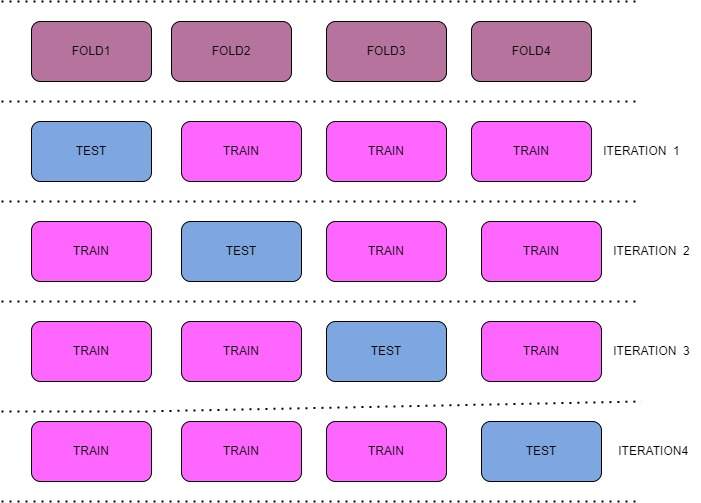
\includegraphics[width=0.8\textwidth]{figure/k-fold.jpeg}
    \caption{Ilustrasi \textit{K-Fold Cross Validation} \cite{comprehensive_bhagat_2025}}
    \label{fig:k-fold}
\end{figure}

Gambar \ref{fig:k-fold} memperlihatkan prosedur sistematis \textit{K-Fold Cross-Validation} dengan membagi dataset menjadi $k$ bagian. Seperti terlihat pada diagram, model dilatih secara berulang sebanyak $k$ kali. Dalam setiap iterasi, $k-1$ bagian (blok train) digunakan untuk pembelajaran, sementara satu bagian yang berbeda (blok test) digunakan untuk validasi secara bergantian. Metode ini memastikan setiap subset data berkontribusi sebagai data uji tepat satu kali, yang menghasilkan estimasi performa model yang lebih akurat dan tidak bias dibandingkan metode pemisahan data sederhana.

\begin{figure}[H] % Kalau menggunakan H, posisi gambar akan tepat dibawah teks
    \centering
    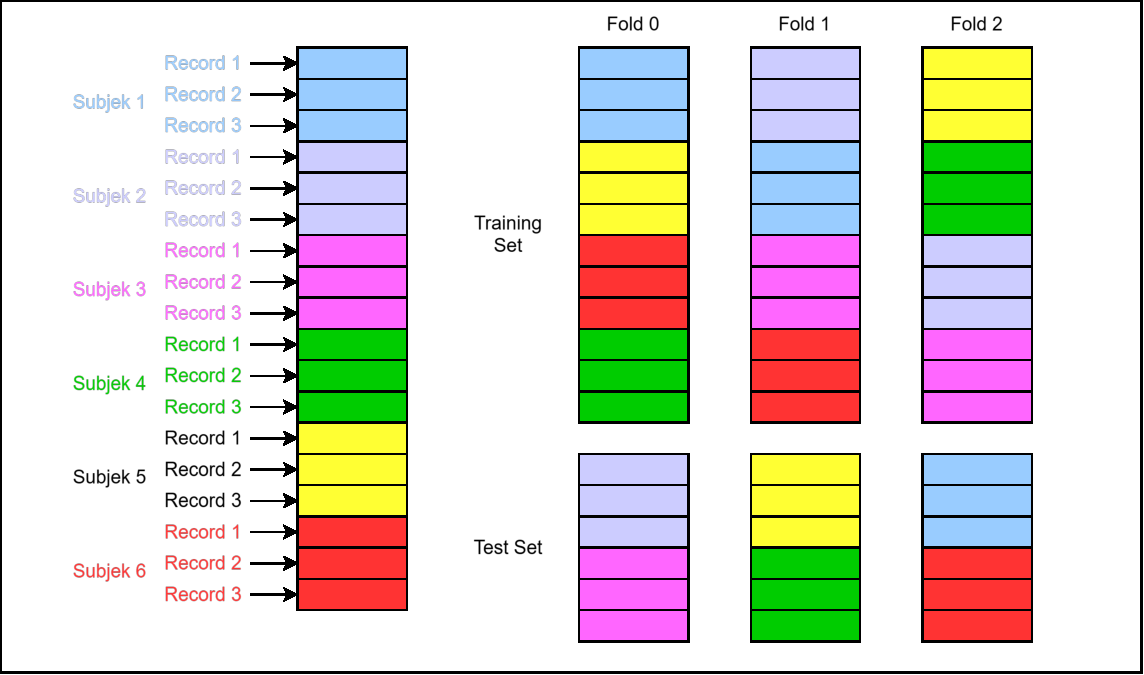
\includegraphics[width=1\textwidth]{figure/k-fold.pdf}
    \caption{Pembagian Dataset dengan teknik \textit{Subject-wise cross-validation}}
    \label{fig:3.pembagian-data}
\end{figure}

Untuk menangani karakteristik data yang kompleks, khususnya pada dataset medis yang memiliki banyak rekaman dari subjek yang sama, diperlukan teknik validasi yang mampu memperhitungkan ketergantungan data antar-subjek. Pada kasus seperti ini, penggunaan \textit{K-Fold Cross-Validation} konvensional berpotensi menghasilkan evaluasi yang bias karena sampel dari satu subjek dapat muncul secara bersamaan pada data latih dan data uji. Oleh karena itu, pendekatan \textit{subject-wise K-Fold Cross-Validation} digunakan, di mana seluruh rekaman yang berasal dari satu subjek ditempatkan secara eksklusif pada satu \textit{fold} yang sama seperti yang terlihat pada gambar \ref{fig:3.pembagian-data}. Pendekatan berbasis subjek ini bertujuan untuk mencegah kebocoran data (\textit{data leakage}) antar-subjek dan memastikan bahwa evaluasi performa model benar-benar mencerminkan kemampuan generalisasi terhadap subjek baru yang belum pernah dikenali sebelumnya \cite{impact_tougui_2021}.

\subsection{Deep Learning} \label{II.Teori1}

\begin{figure}[H] % Kalau menggunakan H, posisi gambar akan tepat dibawah teks
    \centering
    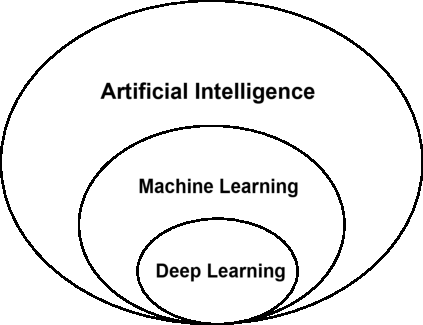
\includegraphics[width=0.6\textwidth]{figure/deeplearn.pdf}
    \caption{Diagram lanskap \textit{Artificial Intelligence}}
    \label{fig:3.ai_lanskap}
\end{figure}

Sebagaimana diilustrasikan dalam diagram lanskap \textit{artificial intelligence} pada \ref{fig:3.ai_lanskap}, \textit{deep learning} bukanlah entitas yang berdiri sendiri, melainkan bagian spesifik dari hierarki sistem cerdas yang lebih besar. AI bertindak sebagai payung utama yang menaungi berbagai pendekatan, termasuk sistem berbasis aturan dan pengetahuan. Di dalam lingkup tersebut, terdapat Machine Learning sebagai subset yang berfokus pada kemampuan belajar dari data, dan \textit{deep learning} hadir secara lebih spesifik di dalamnya sebagai metode yang terspesialisasi, menandakan posisinya sebagai evolusi teknik yang lebih mendalam dari pembelajaran mesin konvensional \cite{ketkar2017deep}.

\textit{Deep learning} adalah cabang dari \textit{machine learning} yang berfokus pada cara komputer memahami data secara bertahap melalui lapisan-lapisan (\textit{layers}) pemrosesan yang disusun secara berurutan. Istilah "deep" atau "dalam" di sini memiliki makna teknis yang sederhana, yaitu merujuk pada jumlah lapisan yang digunakan dalam model jaringan saraf untuk mengolah data, bukan pada kedalaman pemahaman yang bersifat filosofis. Secara prinsip, metode ini bekerja layaknya proses penyaringan informasi bertingkat, di mana data mentah dimasukkan dan diproses melewati banyak lapisan, sehingga di setiap lapisannya data tersebut menjadi semakin "bersih" dan mudah dipahami oleh komputer untuk menyelesaikan tugas yang rumit \cite{chollet2021deep}. 

Dalam \textit{deep learning}, komputer memproses informasi secara bertingkat menggunakan model yang disebut jaringan saraf. Meskipun namanya terdengar biologis dan ide awalnya memang terinspirasi dari otak manusia, sebenarnya teknologi ini tidak meniru cara kerja otak kita sama sekali. Anggapan umum yang sering muncul bahwa \textit{deep learning} bekerja persis seperti pikiran manusia adalah salah kaprah. Sederhananya, \textit{deep learning} hanyalah sebuah kerangka matematika untuk mempelajari data \cite{chollet2021deep}.

\subsection{State Space Models (SSM)} \label{II.Teori1}
State Space Models (SSM) adalah kerangka kerja matematis berprinsip yang digunakan untuk memodelkan dan menganalisis deret waktu (\textit{time series}), seperti data penjualan atau pola cuaca. Inti dari SSM adalah konsep keadaan laten (\textit{latent state}), yang merupakan sekumpulan variabel tersembunyi yang berevolusi seiring waktu dan merekam informasi penting tentang deret waktu, seperti tren dan musiman. SSM didefinisikan oleh dua persamaan: Persamaan Transisi Keadaan, yang menjelaskan bagaimana keadaan laten berubah dari waktu ke waktu, dan Model Observasi, yang menjelaskan bagaimana data yang kita  observasi dihasilkan dari keadaan laten tersebut. Kerangka ini disukai karena kemampuannya untuk dapat diinterpretasi dan efisien data, meskipun secara tradisional model ini diterapkan secara terpisah pada setiap deret waktu \cite{deep_rangapuram_2018}.

SSM didefinisikan oleh dua persamaan utama:
\begin{enumerate}
    \item Persamaan Transisi Keadaan (\textit{State-Transition Equation}): Menjelaskan dinamika transisi stokastik $p(l_t|l_{t-1})$ yang dengannya keadaan laten berevolusi seiring waktu \cite{deep_rangapuram_2018}. Dalam konteks linier, ini seringkali berbentuk:
	\\[5pt]
    \begin{equation}
        l_{t}=F_{t}l_{t-1}+g_{t}\epsilon_{t} \quad \dot{\epsilon}_{t}\sim\mathcal{N}(0,1) \label{eq:ssm-transition}
    \end{equation}
    \myequations{Rumus Persamaan Transisi Keadaan}
    \vspace{1em}

    Di mana $F_{t}$ adalah matriks transisi deterministik, dan $g_{t}\epsilon_{t}$ adalah inovasi acak \cite{deep_rangapuram_2018}.

    \item Model Observasi (\textit{Observation Model}): Menentukan probabilitas bersyarat $p(z_t|l_t)$ dari observasi ($z_t$) yang diamati (data aktual) yang diberikan oleh keadaan laten \cite{deep_rangapuram_2018}.
\end{enumerate}

\subsection{Selective State Space Models}
\textit{Selective State Space Models} (Selective SSM) merupakan pengembangan dari \textit{Structured State Space Models} (SSMs) konvensional yang dirancang untuk mengatasi kelemahan model \textit{Linear Time Invariant} (LTI) dalam menyeleksi informasi yang relevan. Berbeda dengan SSM biasa yang parameter dinamikanya konstan terhadap waktu, Selective SSM memperkenalkan mekanisme seleksi yang membuat parameter model menjadi fungsi dari input itu sendiri (\textit{input-dependent}).

\begin{figure}[H]
    \centering
    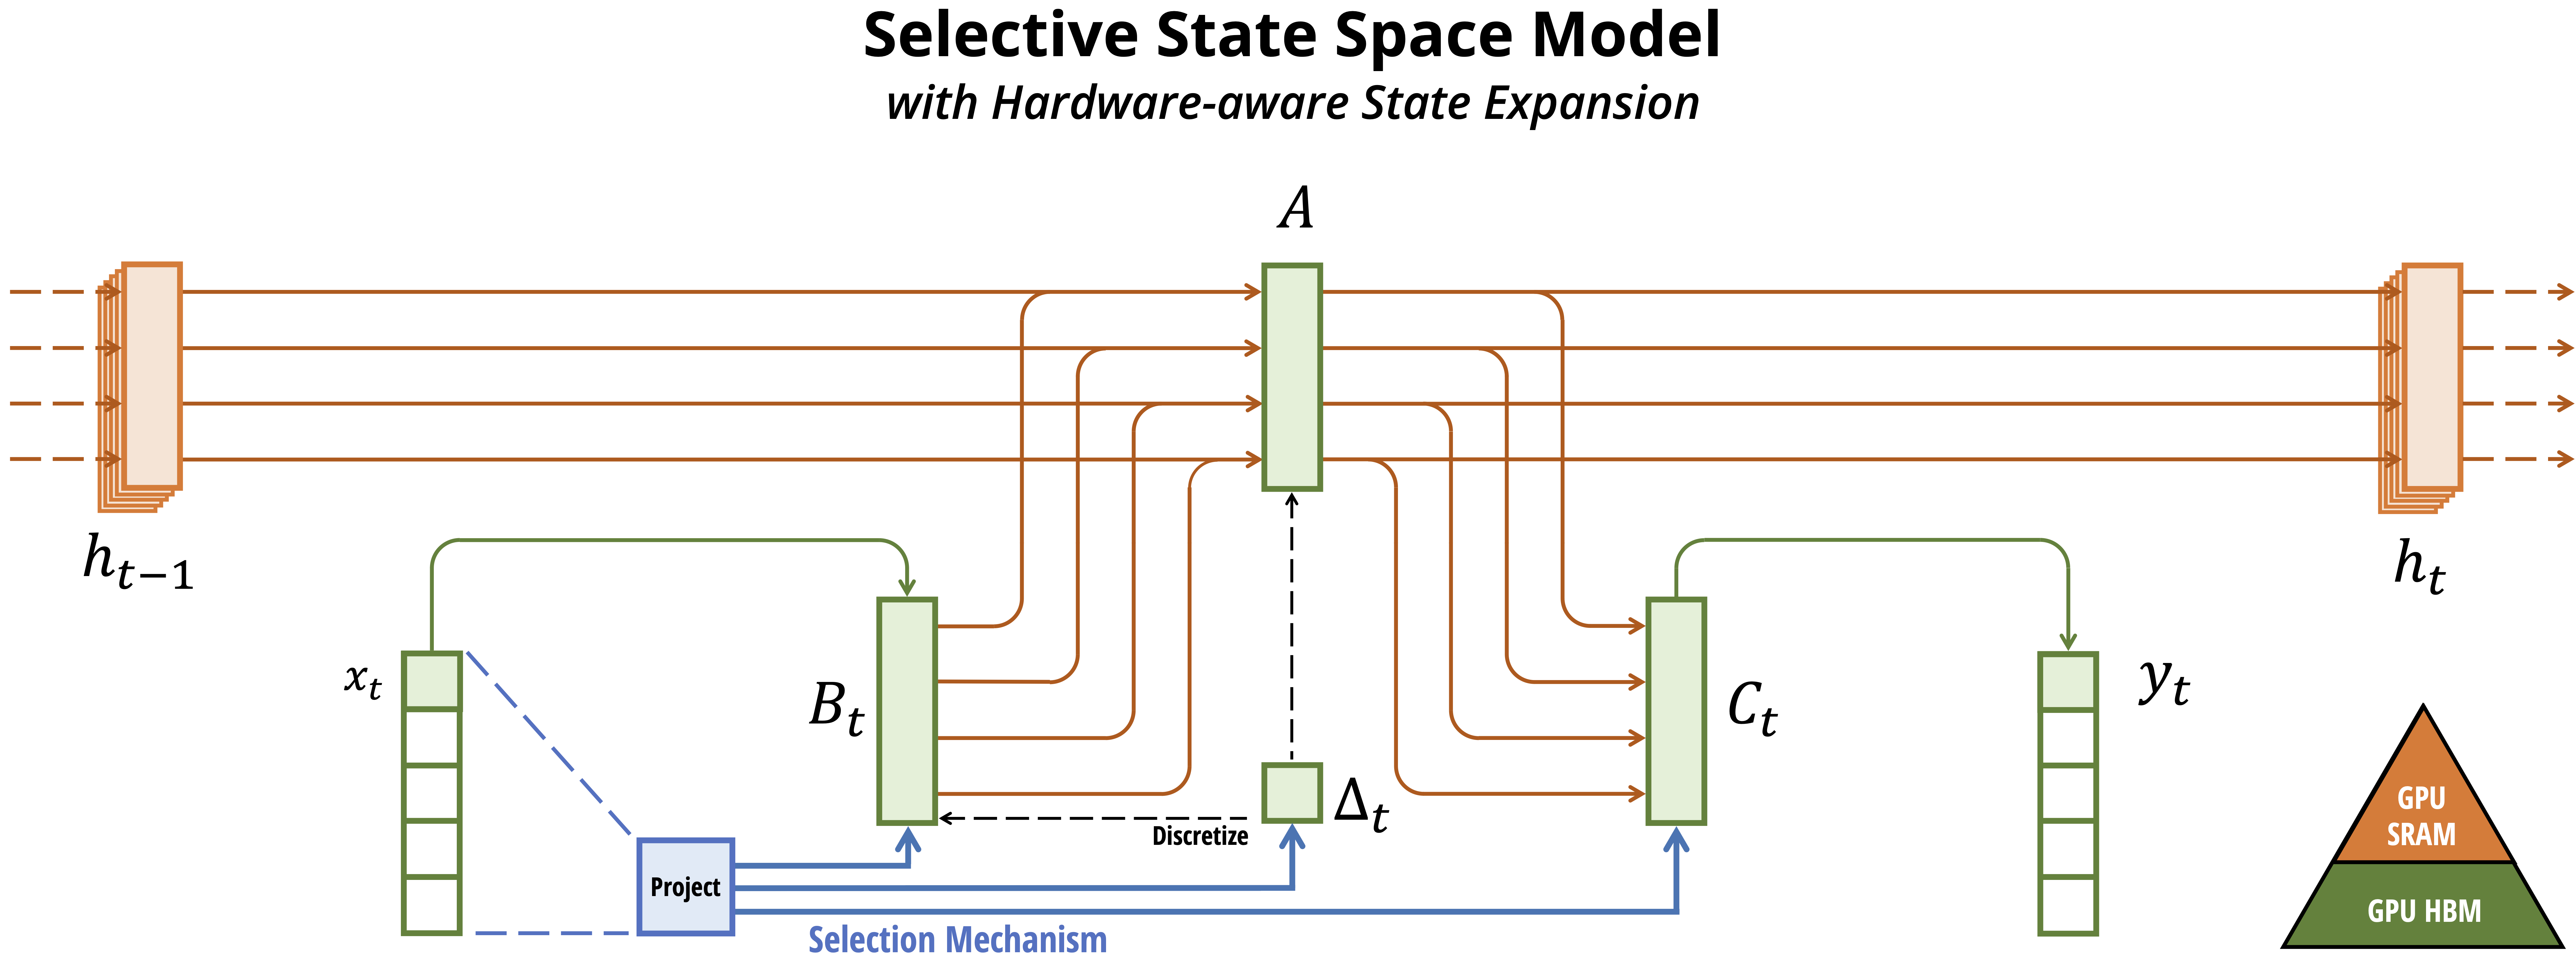
\includegraphics[width=\textwidth]{figure/selection.png}
    \caption{Arsitektur Selective State Space Model \cite{Gu2023}}. 
    \label{fig:selective_ssm}
\end{figure}

Sebagaimana diilustrasikan pada Gambar \ref{fig:selective_ssm}, mekanisme seleksi bekerja dengan mengambil input $x_t$ dan memproyeksikannya untuk menghasilkan parameter dinamis yang memungkinkan model secara selektif mempropagasikan atau melupakan informasi di sepanjang dimensi urutan. Karena perubahan parameter ini mencegah penggunaan konvolusi yang efisien, Selective SSM menerapkan algoritma \textit{hardware-aware}. Seperti yang ditunjukkan pada diagram memori di Gambar \ref{fig:selective_ssm}, algoritma ini menghitung model secara berulang (\textit{recurrent}) menggunakan pemindaian (\textit{scan}), namun tidak mematerialisasikan \textit{state} yang diperluas ($h_t$) ke dalam memori HBM GPU yang lambat, melainkan memprosesnya di level memori SRAM yang lebih efisien untuk menghindari hambatan I/O \cite{Gu2023}.

\subsection{Mamba}
Mamba adalah arsitektur jaringan saraf tiruan baru yang dirancang untuk mengatasi inefisiensi komputasi arsitektur Transformer pada urutan data yang sangat panjang. Secara umum, Mamba adalah model sekuensial yang bekerja dalam waktu linear (\textit{linear-time sequence modeling}), dibangun di atas komponen inti yang disebut \textit{Selective State Space Models} (SSMs), tanpa menggunakan modul attention atau blok MLP (\textit{Multi-Layer Perceptron}) yang biasanya ada di Transformer. Inovasi utamanya adalah membuat parameter SSM bergantung pada input data, yang memungkinkan model untuk secara adaptif memilih  informasi mana yang harus disimpan  dan mana yang harus dilupakan berdasarkan token saat ini. Kemampuan selektif ini secara efektif memungkinkan penalaran berbasis konten yang sebelumnya menjadi kelemahan model subkuadratik lainnya, menghasilkan inferensi yang cepat dan kinerja yang kompetitif di berbagai modalitas, termasuk bahasa \cite{Gu2023}.

\begin{figure}[H]
    \centering
    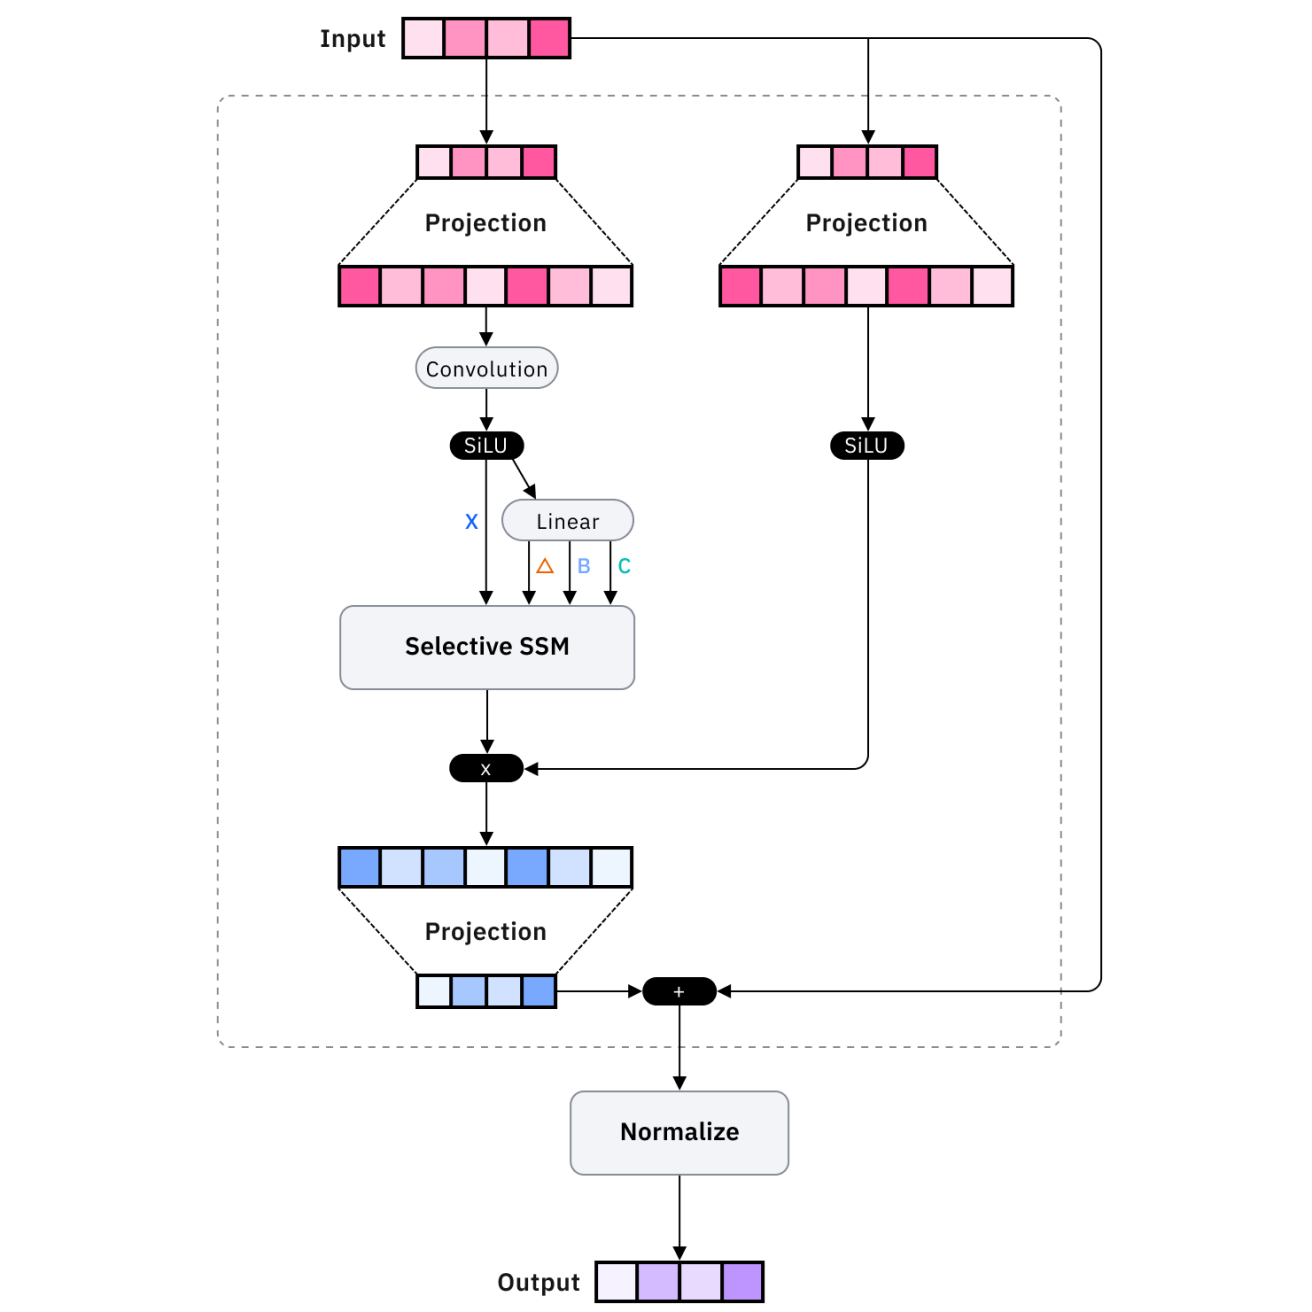
\includegraphics[width=1\textwidth]{figure/mamba_arch.png}
    \caption{Diagram Blok Arsitektur Mamba \cite{ibm2024mamba}}
    \label{fig:mamba_arch}
\end{figure}

Sebagaimana diperlihatkan pada Gambar \ref{fig:mamba_arch}, desain blok Mamba mengadopsi struktur \textit{Gated MLP}. Proses dimulai dengan input yang diproyeksikan ke dimensi yang lebih besar (biasanya dengan faktor ekspansi $E=2$) melalui lapisan \textit{Linear Projection} ke dalam dua cabang paralel. 
\begin{itemize}
    \item Cabang Utama (Kiri): Data melewati konvolusi 1D pendek (\textit{Convolution}) untuk menangkap ketergantungan lokal, kemudian melewati fungsi aktivasi SiLU. Setelah itu, sinyal masuk ke inti \textit{Selective SSM}, di mana parameter $B, C,$ dan $\Delta$ dihitung berdasarkan input (mekanisme seleksi) untuk memproses urutan secara rekursif.
    \item Cabang Gating (Kanan): Cabang ini berfungsi sebagai mekanisme gerbang (\textit{gate}), di mana data diproyeksikan dan melewati fungsi aktivasi SiLU.
\end{itemize}

Output dari kedua cabang ini kemudian digabungkan melalui operasi perkalian \textit{element-wise}, yang menggantikan mekanisme atensi tradisional. Hasil akhirnya diproyeksikan kembali ke dimensi model asli melalui lapisan \textit{Linear Projection} terakhir dan ditambahkan dengan koneksi residual (simbol $+$) untuk stabilitas pelatihan. Struktur ini memungkinkan Mamba beroperasi sebagai \textit{Recurrent Neural Network} (RNN) saat inferensi, memberikan kecepatan yang jauh lebih tinggi dibandingkan Transformer \cite{ibm2024mamba}.

\subsection{\textit{Weighted Cross Entropy Loss}}
Pada permasalahan klasifikasi dengan distribusi kelas yang tidak seimbang, penggunaan fungsi \textit{loss} standar seperti \textit{Cross-Entropy} cenderung menghasilkan model yang bias terhadap kelas mayoritas. Hal ini disebabkan karena \textit{Cross-Entropy} memperlakukan setiap sampel secara setara tanpa mempertimbangkan frekuensi kemunculan masing-masing kelas, sehingga kesalahan pada kelas minoritas memberikan kontribusi yang relatif kecil terhadap total nilai \textit{loss} selama proses pelatihan.

Untuk mengatasi permasalahan tersebut, \textit{Weighted Cross-Entropy Loss} diperkenalkan sebagai pendekatan berbasis biaya (\textit{cost-sensitive learning}) dengan memberikan bobot yang berbeda pada setiap kelas. Dengan cara ini, kesalahan prediksi pada kelas minoritas akan diberi penalti yang lebih besar, sehingga model terdorong untuk mempelajari representasi yang lebih seimbang antar kelas. Secara umum, \textit{Weighted Cross-Entropy} dapat dirumuskan sebagai berikut.

\begin{equation}
\mathcal{L}_{WCE} = - \sum_{c=1}^{C} w_c \, y_c \log(\hat{y}_c),
\end{equation}
\myequations{Rumus \textit{Weighted Cross-Entropy}}
\vspace{1em}

di mana $w_c$ merupakan bobot untuk kelas ke-$c$, $y_c$ adalah label ground truth dalam bentuk \textit{one-hot encoding}, dan $\hat{y}_c$ adalah probabilitas prediksi model untuk kelas ke-$c$.

Phan dan Yamamoto menunjukkan bahwa pemberian bobot pada \textit{Cross-Entropy Loss} merupakan cara yang sederhana namun efektif untuk meningkatkan performa klasifikasi pada kelas minoritas tanpa memerlukan modifikasi arsitektur model atau teknik penyeimbangan data secara eksplisit. Hasil eksperimen mereka pada dataset dengan ketimpangan kelas yang tinggi menunjukkan bahwa \textit{Weighted Cross-Entropy} mampu meningkatkan performa kelas minoritas secara signifikan, sementara performa keseluruhan tetap terjaga dibandingkan dengan \textit{Cross-Entropy} standar \cite{resolving_phan_2020}.

\subsection{\textit{Confusion Matrix}} \label{II.Teori1}
\textit{Confusion matrix} adalah teknik evaluasi yang mendetail dan komprehensif untuk mengukur kinerja model klasifikasi dalam pembelajaran mesin (\emph{supervised learning}) \cite{sathyanarayanan2024confusion}. Konsep ini, yang awalnya dikembangkan oleh Karl Pearson pada tahun 1904 sebagai tabel kontingensi, direpresentasikan sebagai matriks persegi berukuran $N \times N$, di mana $N$ mewakili jumlah kelas output. Matriks ini memvisualisasikan perbandingan antara label kelas sebenarnya (\emph{ground truth}) dengan label yang diprediksi oleh model. Dalam struktur ini, elemen-elemen pada diagonal utama menunjukkan jumlah prediksi yang benar, sementara elemen di luar diagonal merepresentasikan kesalahan klasifikasi atau \emph{misclassification}. Keunggulan utama dari \emph{confusion matrix} adalah kemampuannya untuk memberikan wawasan mendalam mengenai perilaku internal pengklasifikasi (\emph{classifier}), mengungkap kelemahan model, serta membedakan jenis kesalahan yang terjadi, seperti \emph{Type I error} (False Positive) dan \emph{Type II error} (False Negative) \cite{sathyanarayanan2024confusion}.

\begin{figure}[H]
    \centering
    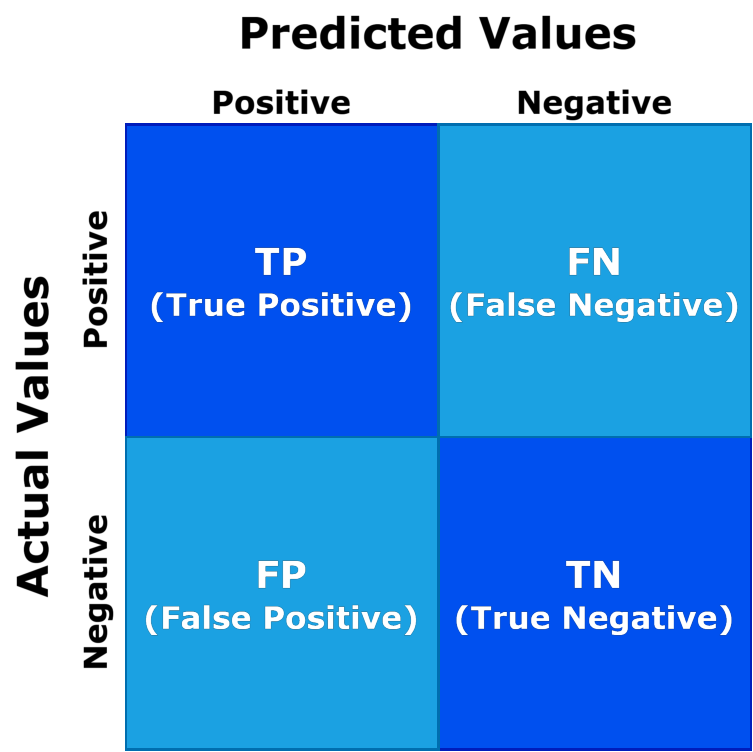
\includegraphics[width=0.7\textwidth]{figure/conf.pdf}
    \caption{Confusion Matrix}
    \label{fig:confusion_matrix}
\end{figure}

Gambar \ref{fig:confusion_matrix} menyajikan visualisasi confusion matrix yang memetakan hasil prediksi model terhadap kelas aktualnya. Informasi yang terkandung dalam matriks ini selanjutnya digunakan sebagai dasar perhitungan untuk berbagai metrik evaluasi kinerja berikut:

\begin{enumerate}
    \item \textit{Accuracy}: Mengukur rasio total prediksi yang benar terhadap keseluruhan sampel data \cite{krstinic2020multilabel}.

    \begin{equation}
        Accuracy = \frac{TP + TN}{TP + FP + TN + FN}
    \end{equation}
    \myequations{Rumus \text{Accuracy}}
    \\[1pt]

    \item \textit{Precision}: Mengukur proporsi prediksi positif yang benar-benar positif. Metrik ini dihitung dengan membagi elemen diagonal dengan jumlah total elemen pada kolom terkait \cite{sathyanarayanan2024confusion}.

    \begin{equation}
        Precision = \frac{TP}{TP + FP}
    \end{equation}
    \myequations{Rumus \textit{Precision}}
    \\[1pt]

    \item \textit{Recall}: Mengukur proporsi kasus positif aktual yang berhasil diidentifikasi dengan benar oleh model. Metrik ini dihitung dengan membagi elemen diagonal dengan jumlah total elemen pada baris terkait \cite{sathyanarayanan2024confusion}.

    \begin{equation}
        Recall = \frac{TP}{TP + FN}
    \end{equation}
    \myequations{Rumus \textit{Recall}}
    \\[1pt]

    \item \textit{F1-Score}: Merupakan rata-rata harmonik (\emph{harmonic mean}) dari presisi dan \textit{recall}. Metrik ini memberikan keseimbangan antara kedua nilai tersebut dan lebih cocok digunakan pada data yang memiliki ketidakseimbangan kelas \cite{sathyanarayanan2024confusion}.

    \begin{equation}
        F1\text{-}score = 2 \times \frac{Precision \times Recall}{Precision + Recall} = \frac{2TP}{2TP + FP + FN}
    \end{equation}
    \myequations{Rumus \textit{F1-Score}}
\end{enumerate}

\subsection{Evaluasi Kompleksitas Komputasi} \label{II.Teori1}
Efisiensi komputasi adalah ukuran seberapa hemat dan cepat sebuah algoritma bekerja, bukan hanya seberapa pintar algoritma itu menebak dengan benar. Evaluasi ini melibatkan analisis kompleksitas waktu, seperti durasi pelatihan dan prediksi, serta kompleksitas ruang yang mengukur konsumsi memori selama operasional model. Selain itu, efisiensi juga dinilai dari optimalisasi pemanfaatan perangkat keras (CPU dan GPU) untuk memastikan algoritma dapat berjalan efektif, terutama dalam lingkungan dengan sumber daya terbatas \cite{sivakumar2024simplified}.

Evaluasi kompleksitas komputasi bertujuan untuk menilai biaya komputasi yang dibutuhkan oleh suatu model pembelajaran mesin dalam proses pelatihan maupun inferensi. Evaluasi ini penting terutama pada pemodelan sekuens panjang sinyal fisiologis, di mana kompleksitas model dapat meningkat secara signifikan. Beberapa metrik yang umum digunakan untuk mengevaluasi efisiensi komputasi meliputi jumlah parameter dan GFLOPs.

\subsubsection{Jumlah Parameter}
Jumlah parameter merujuk kepada total variabel internal yang ada pada sebuah model, terutama bobot (\textit{weight}) dan bias yang nilainya dipelajari dan diperbarui selama proses pelatihan untuk meminimalisir \textit{loss function}. Jumlah parameter sering digunakan sebagai indikator utama untuk mengukur kapasitas memori model serta kompleksitas komputasi yang diperlukan, di mana peningkatan jumlah parameter biasanya berkorelasi dengan peningkatan performa model namun juga meningkatkan biaya pelatihan dan latensi inferensi \cite{10.1145/3578938}.

Perhitungan jumlah parameter bergantung pada jenis lapisan (layer) yang digunakan dalam arsitektur jaringan. Untuk lapisan konvolusi (convolutional layer), jumlah parameter dihitung berdasarkan ukuran kernel, jumlah filter input, dan jumlah filter output dengan rumus sebagai berikut \cite{DBLP:journals/corr/abs-2103-05251}. 

\begin{equation}
    \text{Params} = K \cdot C^2 \cdot D + K
\end{equation}
\myequations{Rumus Perhitungan Jumlah Parameter untuk lapisan konvolusi}
\vspace{1em}

Di mana: $K$ adalah jumlah filter, $C$ adalah ukuran spasial kernel, dan $D$ adalah kedalaman atau jumlah \textit{channel input}.

Sementara itu, untuk lapisan \textit{fully connected}, jumlah parameter adalah hasil perkalian antara ukuran input ($I$) dan ukuran output ($O$) ditambah dengan bias \cite{DBLP:journals/corr/abs-2103-05251}.

\begin{equation}
    \text{Params} = (I \cdot O) + O
\end{equation}
\myequations{Rumus Perhitungan Jumlah Parameter untuk lapisan \textit{fully connected}}

\subsubsection{GFLOPs}
FLOPs (\textit{Floating Point Operations}) adalah satuan metrik standar yang digunakan untuk mengukur kompleksitas komputasi atau "biaya" operasional dari sebuah model \textit{Deep Learning}. Secara teknis, metrik ini menghitung total operasi matematika dasar, khususnya perkalian dan penjumlahan pada bilangan desimal yang harus dilakukan model saat melakukan inferensi atau selama pelatihan \cite{DBLP:journals/corr/abs-2103-05251}.

Karena total operasi pada model yang kompleks sering kali mencapai angka miliaran, penggunaan satuan dasar FLOPs menjadi tidak praktis, sehingga representasinya sering dikonversi ke dalam skala yang lebih besar seperti GFLOPs (\textit{Giga Floating Point Operations}). GFLOPs merepresentasikan jumlah miliar operasi \textit{floating-point} yang dieksekusi, yang berfungsi sebagai indikator utama untuk mengukur kompleksitas komputasi dan efisiensi model pada berbagai platform perangkat keras \cite{10.1371/journal.pone.0324439}. Dalam evaluasi model, nilai GFLOPs yang lebih rendah menandakan model yang lebih ringan dan membutuhkan daya komputasi yang lebih sedikit, sehingga lebih ideal untuk penerapan \textit{real-time} atau pada perangkat dengan sumber daya terbatas.

\subsection{\textit{Mean Absolute Error} (MAE)}
Dalam konteks pemodelan regresi, pengukuran kesalahan rata-rata (\textit{average error}) merupakan hal yang esensial untuk mengevaluasi kinerja model. \textit{Mean Absolute Error} (MAE) atau yang juga dikenal sebagai \textit{L1 Loss}, merupakan ukuran kesalahan rata-rata yang paling alami (\textit{natural}) dan tidak ambigu (\textit{unambiguous}) jika dibandingkan dengan metrik lain seperti \textit{Root Mean Square Error} (RMSE) \cite{willmott2005advantages}. 

Perhitungan MAE secara konseptual sangat sederhana dan transparan, yaitu dengan menjumlahkan magnitudo atau nilai mutlak (\textit{absolute value}) dari setiap kesalahan prediksi individual, kemudian membaginya dengan jumlah total sampel. Secara matematis, formulasi MAE dapat dirumuskan sebagai berikut:

\begin{equation}
    MAE = n^{-1} \sum_{j=1}^{n} |e_j|
\end{equation}
\myequations{Rumus \textit{Mean Absolute Error} (MAE)}
\vspace{1em}

di mana $n$ adalah jumlah total observasi, dan $e_j$ adalah nilai kesalahan (\textit{error}) individual pada sampel ke-$j$. Nilai kesalahan $e_j$ sendiri secara spesifik didefinisikan sebagai selisih antara nilai estimasi atau prediksi model ($P_j$) dengan nilai observasi aktual ($O_j$), yang direpresentasikan dengan $e_j = P_j - O_j$ \cite{willmott2005advantages}.
